\chapter{Materials and Methods}
\label{chapter:methods}

From now on are presented the data and models used for experiments, and how those nowcasting models were verified. The training, validation and verification datasets are presented in Section \ref{section:data}. The baseline CNN (RainNet) model is described in Section \ref{section:rainnet}, and the BCNN Bayesian extension as well as its implemented variants are described in Section \ref{section:bcnn}. After these models are trained, predictions are calculated for 3 hours with the BCNN variants and all baselines models of Sections \ref{section:det_model} and \ref{section:prob_model}. After that, deterministic verification metrics described in Section \ref{section:det_metric} are computed for the predictions of deterministic models and probabilistic model prediction ensemble averages. Then, probabilistic metrics from Section \ref{section:prob_metric} are calculated for the predictions of BCNN and probabilistic models of Section \ref{section:prob_model}. The metrics are then averaged over the test set for each leadtime of interest and visualized. Additional details on the common training procedure of the DL models are described in Section \ref{section:hyper}, and additional details on prediction and metric calculations in Section \ref{section:exp}. Lastly, the software and various resources used are presented in Section \ref{section:software}.


\section{Dataset and Data Selection}
\label{section:data}

As input data, lowest elevation angle radar reflectivity composites with original 1km spatial resolution and 5 minute temporal resolution from the Finnish Meteorological Institute, cropped into a 512x512 km region covering southern Finland are used. The inputs are in this work \textit{downsampled once, lowering the image size to $256 \times 256$ pixels and the effective spatial resolution to 2km}. The domain and bounding box are illustrated in Figure \ref{fig:domain}. The radar network consists of C-band dual polarization radars. 

Because lowest elevation angle horizontal reflectivity is a good estimator of precipitation at ground level, it is a natural data choice for building a nowcasting model. Radar composites archived from these radar scans are readily available at FMI which facilitated their retrieval for this work. Although the bounding box covering southern Finland did have some data quality issues, it was still deemed to be the best choice, when compared to other candidate datasets such as TAASRAD19 \cite{franch_taasrad19_2020}, as the problems were minor and did not disturb the training process. For example, missing pixels were correctly labeled, which allowed trivial removal of composites with some included. 

Some of the problems with the chosen data are related to insufficient data quality control. Specifically, polarimetric information was not used, making the removal of non-meteorological echos less accurate. Also this absence means that attenuation correction could not be performed, having for effect that echoes originating from behind other strong echoes are attenuated and are shown as weaker than they really are. This is partly mitigated by having multiple radars in the composite, but it does not cover all needed scenarios. Another problem with data quality is that even though summer months in southern Finland were chosen making the precipitation likely rainfall, it can not be said for sure as the phase of precipitation in the dataset was not checked. Again, this could have been checked with polarimetric information.


%All of these factors contributed to the choice of the data source. 
%such as TAASRAD19 - removed

The dataset was chosen so that at first, a selection of rainy days were chosen as to correspond to the 100 days with the most pixels exceeding a 35 dBZ reflectivity threshold during the summer period spanning from May to September during years 2019, 2020, and 2021. The present threshold was chosen as a value which convective storms usually exceed during their whole lifetime \cite{voormansik_thunderstorm_2017}, as the events that are of the most interest in the context of this work are such convective storms. Because the dataset used for this work is concentrated to summer months in southern Finland, all precipitation from the dataset is assumed to be rainfall from now on (which is mostly a valid assumption, except for exceptional hail), and the terms will thus be used interchangeably. 

This dataset is then cleaned and filtered, after which it is divided into training, validation, and test sets. Cleaning the data involves first going through all timestamps and removing those with either partially or completely missing data. The filtering part consists of removing timestamps with less than 1\% of pixels containing reflectivity values exceeding 20 dBZ. Splitting of data into training, validation, and testing sets is performed by using a block sampling strategy \cite{schultz_can_2021} with 6 hour long blocks to prevent autocorrelation between consecutive radar images from invalidating independence between splits. The final split sizes were 15840 radar images for the training split, 2664 for the validation split, and 2448 for the test split. The radar images are always downsampled one time using average-pooling before being used in this work. This is done to alleviate the computational load of training and making predictions. As a consequence, the dimensions of the images drops to $256 \times 256$ and their effective spatial resolution then becomes two kilometers instead of one kilometer for full-scale composites. 

% data transformation to dbz , to RR 
% how was data read: PGM, hdf5 datasets made
% hwo was read : 4 at a time 


%Radar composites are stored as gzip-compressed PGM composite files holding uint8 values, which are converted to reflectivity (dBZ) by applying the relation $\text{pixel\_value}_{\text{dBZ}} = -32 + 0.5 * \text{pixel\_value}_{\text{uint8}}$. 

%When fed into neural networks, the composites are read from HDF5 files as this improves reading speed on distributed storage systems. 

From radar reflectivities, rainrate estimates were calculated using Eq. \eqref{eq:z-r} solved for $R$. In this work, Empirically determined Z-R relationship parameters from \citet{leinonen_climatology_2012} are used, where $A=223$ and $b=1.53$. Finally, $z = 10^{Z / 10}$, giving a formula of

\begin{equation}
\label{eq:dbz_to_r}
R = (10^{Z / 10} / 223)^{1/1.53}
\end{equation}
%
for estimating the rainrate $R$ (mm/h) from reflectivities $Z$ (dBZ) with the current FMI data. 

\begin{figure}
	\centering
	%\missingfigure[figwidth=12cm, figheight=10cm]{FMI radar domain, bbox}
	\includegraphics[scale=1.2]{images/domain/fmi_domain}
	\caption{FMI radar domain and the chosen bounding box covering southern Finland. The three letter codes identify the radars, inner circles their worst case effective range (usu. during summer), and outer circles their best case effective range (usu. during winter). The lowest level reflectivity composite from the 30th of June 2020 at 00:05:00 is depicted on the right.}
	\label{fig:domain}
\end{figure} 


\section{Model}

\subsection{The Baseline: A U-Net Based CNN}
\label{section:rainnet}


For the implementation of the Bayesian Convolutional Network the same architecture as for RainNet by \citet{ayzel_rainnet_nodate} is used. Being itself heavily inspired by U-Net and SegNet model families, RainNet adopts a U-shaped encoder-decoder architecture just like them. The encoder is composed of successive intertwined pooling and convolutional layers, reducing image sizes passed to the next layer while increasing the number of filters. The decoder part adopts a mirror architecture of successive upsampling and convolutional layers, increasing the image size while reducing the number of filters. There are five levels in the encoder-decoder structure, just like in SegNet. Additionally, there are skip connections from the encoder to the decoder branch, carrying higher-level filter maps through, just like in U-Net. This is done to counteract the loss of smaller spatial scale details occurring with pooling. The network architecture is presented in Figure \ref{fig:rainnet}.

\begin{figure}[h]
	%\missingfigure[figwidth=12cm, figheight=8cm]{RainNet architecture diagram with vector graphics}
	\centering
	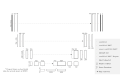
\includegraphics[scale=1]{images/rainnet_arch/rainnet_arch}
	\caption{The functional CNN architecture used for this work, identical to that of RainNet from Ayzel et al. \cite{ayzel_rainnet_nodate}. \texttt{concat} refers to the concatenation of feature maps along the channel dimension.}
	\label{fig:rainnet}
\end{figure}

The convolutional filters have a filter size of three, with padding designed to preserve image shape, and a stride of one. Finally, the last convolutional layer in the network has a filter size of one with no padding, and it is followed by a linear activation output layer, i.e. no (nonlinear) activation function. The network does not contain any fully-connected layers, and in total consists of 31.4M parameters. RainNet works by feeding in four consecutive radar images, with the physically speaking temporal dimension represented in the channel dimension of the tensor. As the output of the network, one image is obtained, representing the predicted frame of the next timestep. In order to make predictions at further leadtimes, the predictions are fed back to the network by appending them to the inputs while removing the oldest image of the sequence in an iterative process. 

The network is trained by calculating a loss function between observed and predicted radar images. This loss function is originally the LogCosh loss in \citet{ayzel_rainnet_nodate}. However in this work, the loss function is swapped for homoscedastic Gaussian Negative Log Likelihood (Gaussian NLL) loss. This is to ensure comparability of the results because it is the loss function used with BCNN. The Gaussian NLL loss \cite{kendall_what_2017} is defined by 

\begin{equation}
\mathcal{L}_\text{Gauss}(y, \hat{y}) = \frac{1}{N} \sum_{i=1}^{N} \frac{1}{2\sigma_\ell^2}||y_i - \hat{y}_i||^2 
+ \frac{1}{2} \log \sigma_\ell^2,
\end{equation}
%
where $i = 1 \dots N$ indexes the number of pixels in the prediction $\hat{y}$ and ground-truth $y$ image or image sequences. Here $\sigma_\ell$ refers to the observational noise parameter. In homoscedastic Gaussian negative log likelihood, aleatoric uncertainty, characterized by $\sigma_\ell$ is assumed to be the same for all data. This parameter can be learned or left constant. In this work, it is tuned using RainNet, by selecting the best value based on validation predictive skill between candidates of $10^{-2}$, $10^{-3}$, and $10^{-4}$. The choices were picked non-rigorously, trying to estimate which order of magnitude would be close to the true uncertainty at different rainrates.

The input rainrates are scaled using a logarithmic transformation $x_{\log} = \ln(x + 0.01)$ as in \citet{ayzel_rainnet_nodate}, after which they are additionally in this work shifted upwards by a factor of five and then scaled down by a factor of 10 to fit into the range of zero to one. The logarithmic transformation of the data is needed because rainrates in themselves are lognormally distributed. This transformation makes them normally distributed, and thus more suitable inputs to neural networks. Additionally, shifting and scaling the inputs to the range from zero to one helps with convergence of RainNet and BCNN. 

Because of the nature of predicting only the next frame, it is very challenging to get a stable nowcast at longer leadtimes. In practice, the precipitation values of nowcasts will often tend to diverge either to zero or infinity. This behavior is alleviated by calculating the loss function for nowcasts done over several leadtimes, which should make the resulting learned network more temporally stable. Hence for training, after pretraining the network with one predicted frame, the training predictions are calculated for a 30 minutes leadtimes (six frames) and the ELBO loss is calculated such that each frame is weighted equally. 

The reason for adopting RainNet as the functional architecture of the Bayesian Neural Network is that compared to for example ConvLSTM based models, it has faster inference without losing much in skill. This is important when building upon a model, especially when having limited resources, as added components make the training and inference slower. 


\subsection{BCNN: a Bayesian Extension to RainNet}

\label{section:bcnn}

BCNN is the Bayesian extension made for this work of the U-Net based architecture described in Section \ref{section:rainnet}. In the network, posterior probability distributions of network parameters are modeled as diagonal Gaussian distributions and optimization is carried out using variants of the Bayes-by-Backprop algorithm described by \citet{blundell_weight_2015}, minimizing the ELBO loss function as described in Section \ref{section:vi}. Posteriors for all parameters are initialized identically to a mean $\mu_q$ of 0 and a variance $\sigma_q$ of $10^{-3}$. Parametrizing the posteriors as Gaussian distributions doubles the number of learnable parameters to 62.8M. Flipout reparametrization \cite{wen_flipout_2018} is used in an attempt to reduce gradient variance and speed-up optimization. 

As for the prior distribution, four variants are implemented. two Gaussian priors having $\mu_P = 0$ and alternatively $\sigma_P = 10^{-1}$ or $\sigma_P = 10^{-3}$, and two Gaussian Scale Mixture (GSM) priors having $\alpha = 0.5$ and alternatively $\sigma_1, \sigma_2 = 3 \times 10^{-1}, 3 \times 10^{-2}$ or $\sigma_1, \sigma_2 = 10^{-1}, 10^{-3}$. The scale-mixture prior might enable faster initialization and more accurate asymptotic behavior, but the Gaussian prior has more convenient mathematical properties, as it enables calculating KL-divergences in closed form when combined with a Gaussian posterior as in here, using the analytical expression

\begin{multline}
D_{\text{KL}}(q(\mathcal{D}|\pmb{w}) || P(\pmb{w})) =\\
\frac{1}{2}\left[\log \frac{|\sigma_P|}{|\sigma_q|}
- d 
+ (\mu_q - \mu_P)^\top \sigma_P^{-1}(\mu_q - \mu_P)
+ tr\{\sigma_P^{-1}\sigma_q\}
\right],
\end{multline}
%
where $q$ and $P$ denote the multivariate diagonal posterior and prior, $\mu_q$ and $\mu_P$ their respective means, $\sigma_P$ and $\sigma_q$ their respective standard deviations and  $d$ the identity matrix of the number of dimensions equal to that of the distributions. 

In BCNN, the radar images undergo the same scaling and preprocessing as described for RainNet in Section \ref{section:rainnet}. The data likelihood cost is modeled as Homoscedastic Gaussian negative log likelihood (NLL) which is the same as the loss function used for RainNet. The $\sigma_\ell$ parameter for BCNN is chosen as the one with the best validation performance with RainNet, based on the ETS metric (see Section \ref{section:det_metric}) at different thresholds, and is kept constant for most experiments afterwards. 

Multiple procedures for weighting the complexity cost against the likelihood cost, some presented in Section \ref{section:vi}, are implemented. In addition to the equal weighting scheme from \citet{graves_practical_2011} abbreviated \texttt{equal} and the batch index dependent scheme from \citet{blundell_weight_2015} abbreviated \texttt{blundell}, a scheme reducing the weight of the complexity cost each epoch abbreviated \texttt{epoch}, defined as $\pi_j = 2^{-j}$, where $j=0,1,\dots$ is the current epoch, is implemented to try and provide potentially better potential asymptotic nowcasting skill. This emanates from the fact that in preliminary experiments, \texttt{equal} has sometimes provided excessive regularization leading to a sub-optimal models, and \texttt{blundell} has had problems with converging when using batch sizes of one or two as is sometimes used in this work.



\begin{figure}[h]
	\begin{center}
		
\includegraphics[scale=1]{images/inference_diagram/inference_diagram.pdf}
		\caption{Inference procedure for generating ensemble nowcasts with the BCNN. Each training sample undergoes the same stochastic iterative procedure independently of one another. The input is in the present work always of dimension $L \times W \times H = 4 \times 256 \times 256$, and the resulting ensemble nowcast of dimension $N \times L \times W \times H = N \times L \times 256 \times 256$, where $N$ could be e.g. one or four in training or 48 in verification, and $L$ one or six in training, or 36 in verification.}
		\label{fig:inference}
	\end{center}
\end{figure}

\begin{figure}[ht]
	\begin{center}
		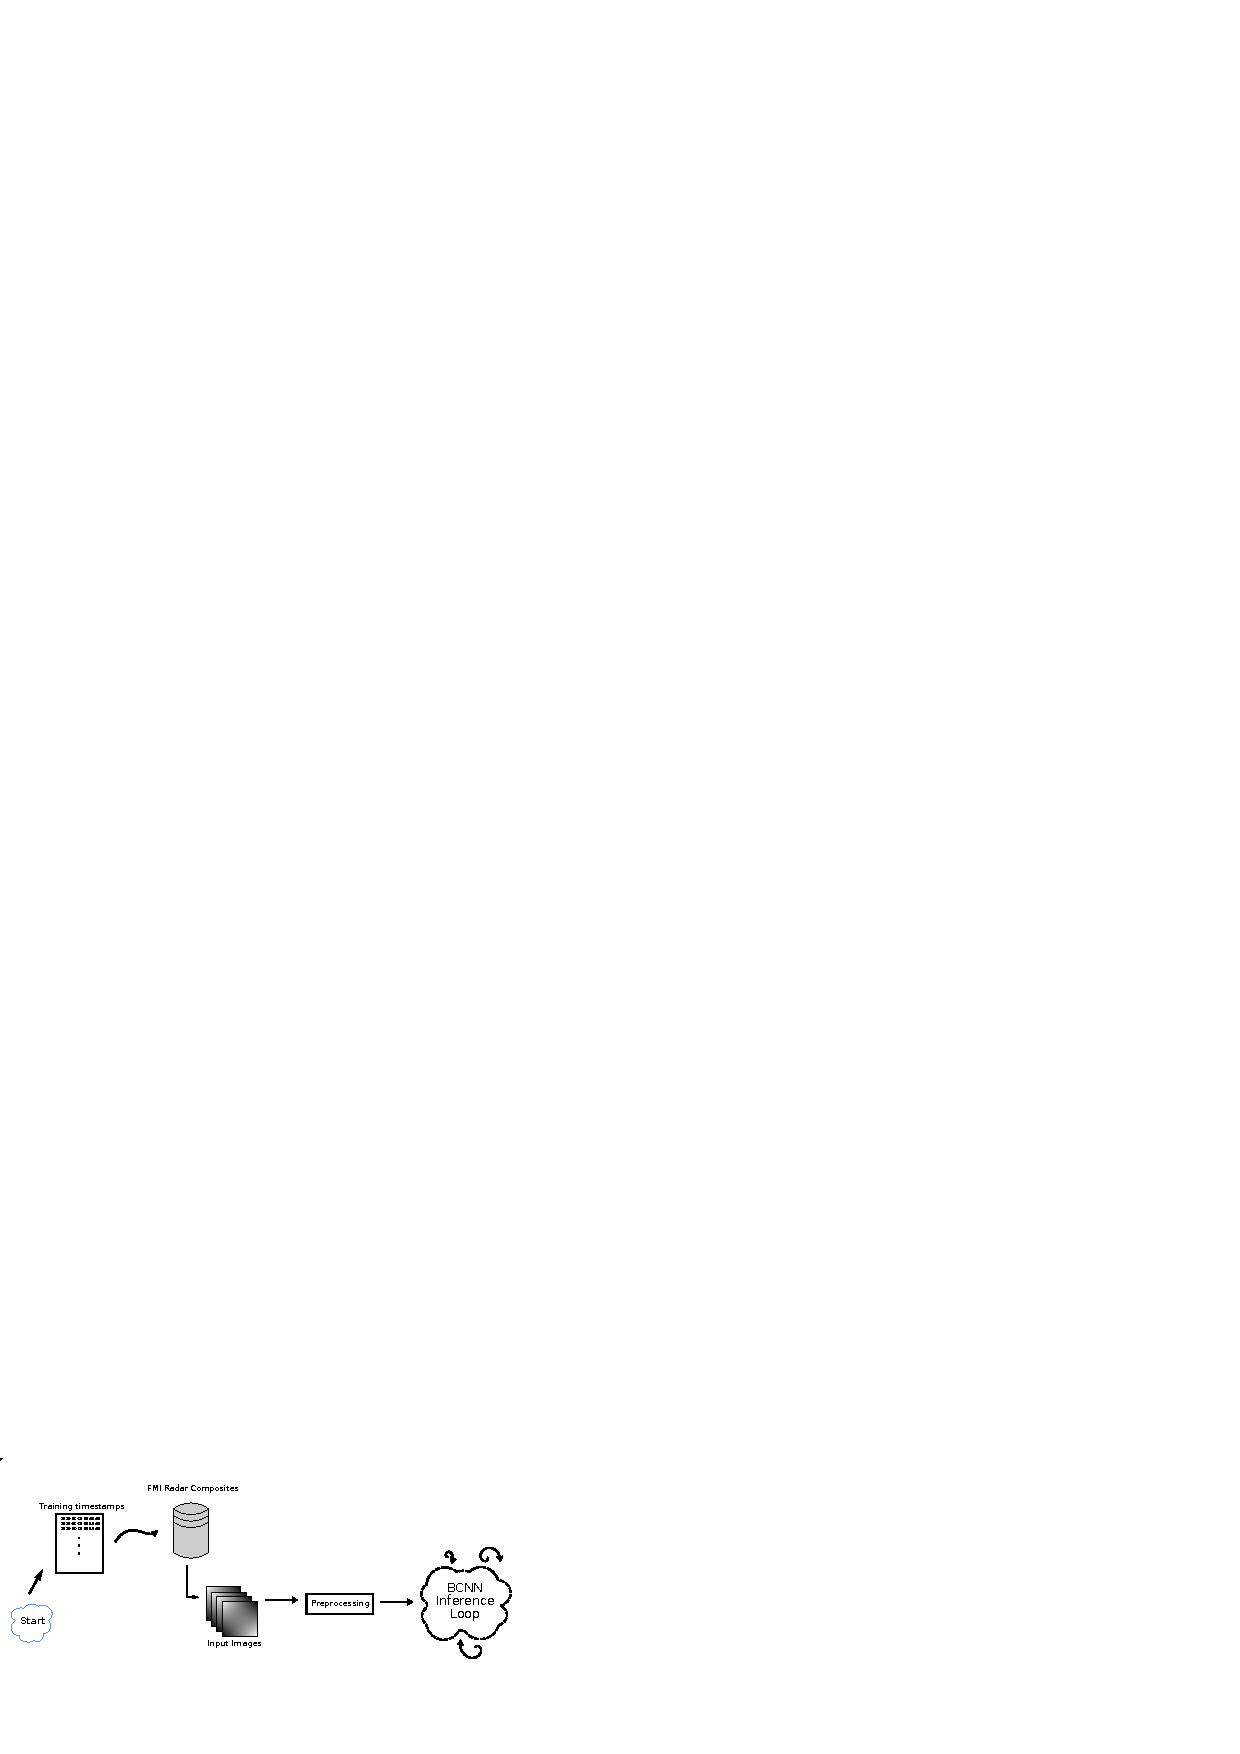
\includegraphics[scale=1]{images/training_diagram/training_diagram.pdf}
		\caption{Training loop for the BCNN illustrated. One loop corresponds to one training minibatch. During the training, the KL-loss of each layer is accessed as a cached property of the network from the previous forward passes. Training sequences formable from successive timestamps are indexed with $i$. Additionally, although oversimplified, $\text{KL}(q \mid \mid p)$ refers in this diagram to the cached complexity cost, $\pi_i$ to the complexity cost weighting associated with the $i$:th sequence, and $\mathcal{L}_{\text{Gauss}}$ to the Gaussian NLL loss.}
		\label{fig:training}
	\end{center}
\end{figure}

%through marginalization over these sampled parameters
With BCNN, predictions are generated by simply doing a forward pass through the network, which samples the parameters and produces a stochastic ensemble member. Predictions for further leadtimes are made in the same way as with the deterministic RainNet, that is by iteratively re-plugging the previous prediction into the network appended to the input sequence, with the oldest image removed. It is important to note that stochasticity is preserved because parameters are re-sampled at each step of the iterative prediction. Ensembles are produced by repeating this process multiple times independently, that is such that one initial ensemble member at timestep $t$ always leads to a no more than a single new ensemble member at the next timestep $t+1$. Sampling is done this way to avoid the problem of exponential growth that would appear if prediction at timestep $t$ would yield more than one new prediction at timestep $t+1$. The inference procedure is illustrated in Figure \ref{fig:inference}.

Training is performed first on a single leadtime (+ 5 minutes), meaning that during one training step, predictions are made and the loss calculated for only one leadtime. After this, the training is continued on six leadtimes, so using predictions until thirty minutes in the future. This is done in an attempt to speed up model convergence compared to training the model on many leadtimes right from the start. At each training step, input images are transformed, after which the inference procedure in Figure \ref{fig:inference} is ran for the data, yielding a prediction ensemble and the complexity cost. Complexity and likelihood costs are averaged over the ensemble, and are used to calculate the ELBO loss and subsequent parameter updates after backpropagation. A diagram illustrating the training process is shown in Figure \ref{fig:training}. 

The model selection process is performed hierarchically as follows: Starting with the optimal Gaussian NLL parametrized by the uncertainty parameter obtained through RainNet training experiments and \texttt{equal} complexity cost weighting, BCNN models with the four selected priors are trained. The best performing model is selected based on the validation likelihood cost, and it is retrained using the \texttt{epoch} and \texttt{blundell} complexity cost weighting. Out of them, the best performing model overall is selected and named \texttt{BCNN lt5}. This model has its training continued with six leadtimes, and the resulting model is called \texttt{BCNN lt30}. After that, an alternative training regime using four training samples (meaning using four-member prediction ensembles for the training) instead of only one is tried for \texttt{lt5}, with the resulting model called \texttt{BCNN lt5 new}. A further experiment for \texttt{lt5} is carried out again with four training samples but this time also with the Gaussian NLL data uncertainty parameter $\sigma_\ell$ set to an alternative, considerably bigger value than the optimal one from the likelihood perspective. This model is called \texttt{BCNN lt5 v2}. The training for that model is also continued for six leadtimes, resulting in \texttt{BCNN lt30 v2}. The batch size is chosen as the biggest power of two fitting into VRAM (32GB). 
Consequently, \texttt{BCNN lt5} is trained with a batch size of 32, \texttt{BCNN lt30}, \texttt{BCNN lt5 new} and \texttt{BCNN lt5 V2} using a batch size of 8, and finally \texttt{BCNN lt30 v2} using a batch size of two.

\subsection{Additional Hyperparameters for the Neural Networks}
\label{section:hyper}

 Both for RainNet and BCNN, the Adam optimizer is used with an initial learning rate of $10^{-4}$ without any learning rate scheduler. For RainNet, other hyperparameters were left to their \texttt{torch.optim.Adam} default values, but for BCNN, the momentum parameter $\beta_1$ was increased to $0.95$ to better accommodate the increased stochasticity of SVI compared to non-Bayesian NN \cite{noauthor_svi_nodate}. Early stopping was set for both models with for condition that the validation loss does not decrease for 3 epochs. For BCNN, only the likelihood part of the loss was taken into account in the early stopping criterion. 


\section{Baseline Models}

In this section are concisely presented all deterministic and probabilistic models used as baselines for benchmarking BCNN skill. The parameters used are stated for ensuring reproducibility, and a short reasoning for the choice of each model is given.

\subsection{Deterministic Models}
\label{section:det_model}

In order to verify the skill of BCNN, multiple deterministic models were used to produce nowcasts against which those produced by BCNN are compared. First and foremost, the ensemble averages of BCNN are compared against those of RainNet trained with both one and six frames for training, with the configuration outlined in Sections \ref{section:rainnet} and \ref{section:hyper}. It is interesting to compare the skill between the classical predictions and Bayesian version ensemble means, as underlying functional architectures and loss functions are the same, with the only change being the effect of the Bayesian prior on training and the uncertainty related to the Gaussian posteriors at evaluation time. 

In addition, predictions were calculated with a few non-deep-learning models introduced in Section \ref{section:classic_nowcast}. These are Lagrangian Persistence (extrapolation nowcast) and LINDA-D, the deterministic version of LINDA. Lagrangian persistence represents in practice 
a very pragmatic baseline because of its ubiquity and simplicity, while having good skill. It is apparent that most (deterministic) models that can claim to be useful have to at least in a certain way outperform Lagrangian Persistence. LINDA-D on the other hand represents one such model, particularly outperforming Lagrangian Persistence on heavy rainfall. In the event that BCNN outperforms Lagrangian Persistence, LINDA-D serves to assess better the degree of performance achieved. 


Concerning baseline models other than RainNet, before all predictions, the bounding box is applied, input data is converted to rainrate using Eq. \eqref{eq:dbz_to_r} and thresholded at 0.1 mm/h and possible NaN values are set to zero. After predictions are made, these are thresholded at 0.1 mm/h and converted to back to reflectivities by first using Eq. \eqref{eq:z-r} with parameters $A$ and $b$ stated in Section \ref{section:data} and then converting Z to dBZ for storage. When predictions are read for metric calculation, they are once again converted to rainrate before metric calculations.

Both extrapolation and LINDA-D, as well as models described in Section \ref{section:prob_model} use Lucas-Kanade optical flow for advection field estimation with Pysteps \cite{pulkkinen_pysteps_2019} 1.6.1 default parameters and four input frames with field interpolation. These models also perform advection using the Semi-Lagrangian backward scheme of Pysteps using cubic interpolation and with other parameters left to default values. LINDA-D has stochastic perturbations set off with the \texttt{add\_perturbations} flag and otherwise uses default parameters. 


\subsection{Probabilistic Models}
\label{section:prob_model}

Probabilistic skill verification was performed against STEPS and LINDA-P. The former was chosen as it is a well-established and broadly used model offering good performance for a relatively low inference cost of 1-2 minutes to produce a 3 hours nowcast of 24-48 ensemble members on a modern CPU for a domain of $512 \times 512$ pixels \cite{pulkkinen_pysteps_2019}. It thus makes sense to want BCNN to perform at least on the same level as STEPS, considering that the time required for inference with it might not be much lower than that. LINDA-P, also known as the probabilistic variant of LINDA, is computationally more expensive but represents the state-of-the-art in terms of probabilistically predicting localized high-intensity rainfall. Consequently, LINDA-P makes for an interesting benchmark for those cases. 

The same preprocessing and postprocessing pipelines as for deterministic cases (Section \ref{section:det_model}) are used with baseline probabilistic models. Also, the same optical flow and extrapolation parameters are used, and again, Pysteps 1.6.1 default values for methods are used unless stated otherwise. 

Probabilistic nowcasts are set to produce 48 ensemble member nowcasts, just as BCNN. STEPS has parameters set to match the input data, that is \texttt{km\_per\_pixel} is $2.0$ and \texttt{timestep} is $5.0$, also \texttt{R\_thr} is set to $-10$. LINDA-P has the same parameters as LINDA-D, except that naturally stochastic perturbations are set to \texttt{True} with the \texttt{add\_perturbations} flag. It has to be noted that using the current configuration, STEPS is set to add advection field stochastic perturbations while LINDA-P does not. This affects the characteristics of the nowcasts generated, making STEPS nowcasts tend to have higher predictive uncertainty than those of LINDA-P.

\section{Verification Visualizations and Metrics}

Here onward are presented the verification metrics and visualization methods used to benchmark the performance of BCNN. The metrics are divided into deterministic and probabilistic ones. Deterministic metrics assess the performance of ensemble prediction means and deterministic predictions, whereas probabilistic metrics take ensemble uncertainty quality into account in their evaluation. This uncertainty estimation quality is also evaluated visually through different images of predictions.

\subsection{Deterministic Prediction Skill Evaluation Metrics}
\label{section:det_metric}

Deterministic prediction skill scores are calculated in order to compare the raw predictive skill of ensemble nowcasts to the skill of deterministic models. Such comparison is an important facet of verification as low skill in deterministic scores would even for an otherwise competent model mean that it would benefit from being complemented by a stronger deterministic model. In the case of ensemble nowcasting, deterministic scores were calculated for ensemble means. Implemented deterministic metrics are divided into four different categories, roughly complementing each others. These are continuous, categorical, and spatial scores, as well as radially-averaged power spectral density.  

Continuous scores scores are as their name suggests distance metrics used for the evaluation of continuously valued predictions, i.e. regression tasks. The continuous scores used are Mean Error (ME) and Mean Absolute Error (MAE), and they are calculated for leadtimes up until two hours. ME is defined as 

\begin{equation}
	\text{ME} = \frac{1}{N}\sum_{i=1}^{N} y_i - \hat{y}_i,
\end{equation}
%
where summation is performed over the $i=1,\dots,N$ pixels in the radar image, $y$ denotes ground truth and $\hat{y}$ the prediction made. The principal utility of Mean Error is detection whether predictions are biased towards too low or too high rainrates at a certain point in time. On the other hand, 

\begin{equation}
	\text{MAE} = \frac{1}{N}\sum_{i=1}^{N} |y_i - \hat{y}_i|,
\end{equation}
%
only cares about the magnitude of the errors in predictions by taking the absolute value, so it gives an idea of the prediction skill over the images \textit{on average}. Nevertheless, this is not enough to accurately assess the skill of a nowcast method, because not all pixels are equally important, as most of them have no rain or very low rainrates that are not interesting to predict. 
\begin{wraptable}{r}{0.6\textwidth}
	\centering
	\begin{tabular}{@{}|c|c|c|@{}}
		
		\toprule
		\textit{\begin{tabular}[c]{@{}c@{}}Precipitation\\ is ...\end{tabular}} &
		\multicolumn{1}{l|}{\textbf{Observed}} &
		\textbf{\begin{tabular}[c]{@{}c@{}}Not\\ observed\end{tabular}} \\ \midrule
		\textbf{Predicted} &
		\cellcolor[HTML]{D9FFD9}\begin{tabular}[c]{@{}c@{}}TP\\ (Hits)\end{tabular} &
		\cellcolor[HTML]{FFCAB1}\begin{tabular}[c]{@{}c@{}}FP\\ (False Alarms)\end{tabular} \\ \midrule
		\textbf{\begin{tabular}[c]{@{}c@{}}Not\\ predicted\end{tabular}} &
		\cellcolor[HTML]{FFCAB1}\begin{tabular}[c]{@{}c@{}}FN\\ (Misses)\end{tabular} &
		TN \\ \bottomrule
	\end{tabular}
	\caption{Contingency table of categories used. Alternative nomenclature is shown in parentheses.}
	\label{table:contingency}
\end{wraptable}


Additionally, A poor forecast may have good MAE and vice versa. To illustrate this, a forecast failing to predict localized intense precipitation, but otherwise accurately capturing light precipitation over large areas will usually have a small MAE but will have low operational usefulness.
This limited utility of continuous scores serves as a motivation to introduce categorical scores. These are based on the principle of comparing the presence or absence of a rain event in observations and predictions as defined by having a pixel exceeding a threshold value $R_{\text{THR}}$. The categorical scores are defined by dividing events into four categories, that are true positives (TP), i.e rain events that were correctly predicted, true negatives (TN), i.e. lack of rain event that was correctly predicted, false negatives (FN), i.e. rain that wasn't successfully predicted, and false positives (FP), i.e rain that was erroneously predicted. These categories and their relations are illustrated in Table \ref{table:contingency}. Scores derived from those quantities that are used are probability of detection (POD) \cite{schaefer_critical_1990} defined as

\begin{equation}
	\text{POD} = \frac{\text{TP}}{\text{TP}+\text{FN}},
\end{equation} 
%
which simply tells the probability that an event really occurring is correctly predicted. Next, false alarm rate (FAR) \cite{schaefer_critical_1990} is calculated as 

\begin{equation}
	\text{FAR} = \frac{\text{FP}}{\text{TP}+\text{FP}},
\end{equation}
%
which reversely indicates the percentage of positively predicted events not actually happening. Critical success index (CSI) \cite{schaefer_critical_1990}, which is defined as 

\begin{equation}
	\text{CSI} = \frac{\text{TP}}{\text{TP}+\text{FN}+\text{FP}}
\end{equation}
%
is computed and aims to generally assess the performance of the forecast by taking the proportion of correct positive event predictions out of critically important cases, that is those excluding true negatives but including both false alarms (FP) and misses (FN). Lastly, the equitable threat score (ETS) \cite{hogan_equitability_2010} is defined as  

\begin{equation}
\begin{split}
\text{ETS} = \frac{\text{TP} - rnd}{\text{TP}+\text{FN}+\text{FP} - rnd}, \\
\text{where } rnd = \frac{(\text{TP}+\text{FN})(\text{TP}+\text{FP})}{\text{TP}+\text{FN}+\text{FP}+\text{TN}}
\end{split}
\end{equation}
%
is computed. ETS aims to improve CSI assessment of forecast skill, by attempting to estimate the amount of random TP among the prediction using the term $rnd$, and remove that number of data points from the calculations.

The $R_{\text{thr}}$ thresholds chosen for the performing verification are 0.5, 5.0, and 20.0 mm/h. 0.5 mm/h corresponds to very light rainfall and should be easy to predict, 5.0 mm/h to moderately heavy rainfall while 20.0 mm/h corresponds to very heavy and rare rainfall, which is very difficult to predict even for short leadtimes. These metrics are calculated for up to two hours leadtimes. 

In addition to evaluating prediction skill above rainrate thresholds, it is also important to be able to evaluate the nowcast predictive performance at multiple spatial scales. The reason for this is that larger spatial scales have more predictability, and so predicting smaller scales is more difficult while also being of high importance in the context of heavy localized rainfall. 

%in fss, we can determine a threshold for acceptable skill to determine the scale at which nowcasts are good wrt lt 

As such, a spatial verification score, namely Fraction Skill Score (FSS) \cite{roberts_scale-selective_2008} is added to the panoply of metrics used. FSS is a verification metric aiming to estimate the prediction skill above a certain threshold at different spatial scales. It works by calculating a binary threshold exceedance map for forecasts and observations, averaging it over gaussian windows of different lengths representing scales, and calculating for each of those a Mean Squared Error (MSE) skill score relative to a reference low-skill forecast \cite{roberts_scale-selective_2008}. FSS is calculated for thresholds of 0.5, 5.0, and 20.0 mm/h and spatial scales of four and 16 kilometers, up until two hours again. 

Last but not least, the ability to maintain small-scale details as the forecast leadtime increases is related to the skill of the nowcast with regards to the spatial scale. Failure in maintaining those details will results in low skill at small scales and a blurred forecast demonstrated by a dip in nowcast small-frequency power spectral density. Hence the last deterministic verification metric chosen is Radially-Averaged Power Spectral Density (RAPSD). This metric as its name suggests provides a way of calculating power spectral densities for 2D images such as nowcasts, independently of direction. RAPSD characterizes the amount and type of blurring occurring in deep-learning based models verified. It is calculated at 15, 60, and 120 minute leadtimes for all predictions and it is compared to observation RAPSD at those instants. 

\subsection{Visual Evaluation of Nowcast Predictive Uncertainty and Skill}
\label{section:viz_methods}

In order to visually assess ensemble nowcasts, ensemble mean and predictive uncertainty equivalent to two standard deviations of nowcasts are visualized and compared to radar observations. These quantities are calculated for prediction ensembles after being converted to rainrate units. In addition, rainrate exceedance probability estimations for the ensemble are visualized for thresholds of 0.5, 5.0, and 20.0 mm/h. Leadtimes chosen for these visualizations include 5, 15, 30, and 60 minutes. This allows to assess visually the evolution of the accuracy and uncertainty of the ensemble from very short to medium-long leadtimes. 

These visualizations are made for two distinct cases from the verification (test) set containing a mix of stratiform and convective rainfall. The first one (Case 1) contains a fast north-moving heterogeneous front, and starts on the 25th of May 2019 at 13:00 local (Helsinki) time. The second one (Case 2), starting on the 18th of May 2021 at 21:00 local (Helsinki) time, represents again a heterogeneous front, but this time it exhibits large scale spinning motion rather than the relatively uniform motion of Case 1. The presence of both types of precipitation serves to assess differences in the developed method with regards to the rainfall type, knowing that convective events should be notoriously harder to predict. Case 1 nowcast examples are presented for \texttt{BCNN lt5}, \texttt{BCNN lt30}, \texttt{BCNN lt5 new}, and the STEPS baseline, whereas a Case 2 nowcast example is only presented for \texttt{BCNN lt5}.

\subsection{Probabilistic Prediction Skill Evaluation Metrics}

\label{section:prob_metric}
Deterministic verification scores are not enough to accurately assess ensemble forecast skill, because the advantage brought by ensembles does not lie in their mean value, but rather in the breath and quality of their distributions, allowing to weight in multiple possible scenarios. Consequently, specialized metrics designed to assess probabilistic forecasts are needed. 
For this work, four different probabilistic metrics are used for verification. These are the Continuous Ranked Probability Score (CRPS), rank histograms, reliability diagrams, and Receiver operating characteristic (ROC) curves. 

CRPS is a metric generalizing MAE for probabilistic forecast. It is defined as 

\begin{equation}
	\text{CRPS}(F,x) = \int_{-\infty}^{\infty} (F(y) - \mathds{1}(x \geq y))^2 \mathrm{d}y, 
\end{equation}
%
where $F$ is the forecast cumulative density function (CDF) and $\mathds{1}(x \geq y)$ is the indicator function, representing the empirical CDF of the observation $x$. CRPS aims thus to represent the distance between those cumulative distributions as a proxy to estimate ensemble forecast skill. 

A rank histogram is a measure that from the rank of the radar observation among ensemble members, builds a histogram. For each pixel, the rank is determined and and a bin is incremented accordingly. The shape of the histogram is indicative of  whether the spread of the ensemble is representative of the true spread of observations. Variability in the ensemble equal to the uncertainty of observations would make a flat histogram. A convex histogram would mean that ensemble spread under-estimates true uncertainty, whereas a concave histogram would mean that uncertainty is over-estimated, that is that the ensemble is more uncertain that it should be. Furthermore, skewness of the histogram gives a hint on whether there is any kind of bias in the predictions of the ensemble. This goes a step further than ME, as it does not simply tell the average error, but estimates its distribution in a sense. 


ROC curves \cite{mason1982model} are a verification method assessing the ability of a forecast to discern between positive and negative events, that is in the present case pixels with or without exceedance of a particular rainrate threshold. This is accomplished by keeping track of false alarm rates (FAR) against probability of detection (POD) of an event. Probabilities are divided into a certain number of bins over which corresponding FAR are averaged, and a curve is formed. A random forecast corresponding to no skill corresponds to a line, and an increasing area under the curve (AUC) indicates better discernment ability.

A reliability diagram presents observed relative frequencies of events (rainrates exceeding a certain threshold value) against their average forecast probabilities. When these two values are close to each others, the forecast is said to be reliable. This means that a reliable forecast is defined as having its reliability diagram close to the straight line corresponding to observed relative frequencies and forecast probabilities output by the model being equal. In practice, reliability diagrams are built by dividing forecast probabilities into bins with associated observed relative frequencies. The diagram is often accompanied by a histogram of event counts in those bins called the sharpness histogram. A model's forecasts can be said to be sharp if most predictions are close to zero or one probabilities. Sharpness can be seen as a measure of the "decisiveness" of a forecast.

ROC curves are conditioned on observation of an event, while reliability diagrams are conditioned on its forecast. Because of this they complement each others well in the evaluation of ensemble prediction skill. For ROC curves and reliability diagrams, the same rain intensity thresholds as in deterministic metrics, namely 0.5, 5.0, and 20.0 mm/h are used. CRPS is calculated for the first 12 timesteps covering leadtimes up until one hour, while other metrics are shown solely for a one hour leadtime. Additionally, the AUC of the ROC curve is shown for all models except LINDA-P for leadtimes of 0.5, 1.0, 5.0, 10.0, 20.0, and 30.0 mm/h and leadtimes of 15, 30, 60, and 120 minutes. Other metrics are calculated and shown for all models, including LINDA-P.

 With all of the scores and visualizations described in Sections \ref{section:det_metric}, \ref{section:viz_methods}, and \ref{section:prob_metric} complementing each other, forecast skill is estimated as their combination, as no single one of them is capable of capturing all of the facets of a skillful nowcast by itself. 
 
\section{Experimental Setup Details}
\label{section:exp}

In order to make sure that results are valid, all timestamps having any (even a single) observation missing are discarded, and similarly timestamps having any prediction from any model missing are also removed from calculations. Additionally, only pixels where data is present in the predictions of all models are counted in metric calculations. This is accomplished by calculating a common NaN (missing value) mask using the logical OR operation over NaN values of each model, and subsequently applying that common mask to each prediction.

Regarding probabilistic nowcasts, uncertainties present in the data are coming from a diverse set of sources, including both aleatoric and epistemic uncertainties. In order to accurately represent the data distribution resulting from this compound uncertainty, a large ensemble size is needed. This is why the ensemble size was chosen to be 48 for all models. Verification might be even more reliable with bigger ensembles, but this would be at the expense of too much storage space needed for predictions, which would be very inconvenient. Chosen sizes were deemed to be a good compromise regarding this dilemma.

Intermediate results are saved such that predictions are saved in HDF5 archives, in a format where each predicted radar image is a separate dataset in deterministic models, and all ensemble members of predicted radar images for a certain leadtime is its separate dataset in ensemble nowcast models. In this storage procedure, predicted float reflectivity values are first compressed into 8-bit unsigned integers with a scale-offset scheme, then thresholded to 0.1 mm/h to facilitate further lossless compression which is finally carried out using GZIP. Trying to reduce the storage space needed is essential because predictions in this work take in total a very large ($>$ 100 GB after these procedures) amount of space on disk. This is a consequence of combining a big number of timestamps, ensemble members and leadtimes for multiple models. Raw metrics (numerical values) do not suffer from the same problem and are saved to disk in a binary Numpy format.  

\section{Software and Resources}

\label{section:software}

The overall workflow of building models and making experiments, along with what software and environment was used for which task, is summarized in Figure \ref{fig:workflow}.

\begin{figure}[ht]
	\centering
	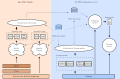
\includegraphics[width=\textwidth]{images/workflow/workflow}
	\caption{Overall workflow showing the process of this work, tied with used libraries for different components. Models and components shown are non-exhaustive.}
	\label{fig:workflow}
\end{figure}

The deep learning models were all implemented using the PyTorch framework and the PyTorch Lightning wrapper \cite{Falcon_PyTorch_Lightning_2019}. These libraries were chosen because of the combined ease of prototyping brought by PyTorch Lightning, and the maturity and flexibility of the parent framework PyTorch. RainNet was ported to PyTorch following the original TensorFlow \cite{abadi_tensorflow_2016} implementation available on Github by \citet{Ayzel2020RainNet}. 

As for the implementation of the probabilistic inference mechanisms for Bayesian Neural Networks, choice was made not to implement them by hand, but to rely on the machinery contained in the Probabilistic Programming Language (PPL) Pyro \cite{bingham2018pyro}, which is itself built on top of PyTorch and includes a fully-featured implementation of Stochastical Variational Inference (SVI). In order to facilitate the implementation task, the TyXe package \cite{ritter2021tyxe} was used. TyXe is a library designed to provide an interface simplifying the implementation of Bayesian Neural Networks using PyTorch and Pyro. A few of the reasons why TyXe was chosen are that it permits easily turning existing neural networks into BNNs without having to use hard-coded bayesian layers, and dynamically switching on-and-off the local reparametrization trick and flipout in layers. Some problems encountered include components of TyXe having difficulties working together with PyTorch Lightning abstractions.

Verification experiments and non-deep-learning baseline models were ran and implemented using the open-source library Pysteps \cite{pulkkinen_pysteps_2019}. It provides implementations for all non-deep-learning models described as well as implementation of verification metric primitives used in this work, and tools for their visualization. 

The computational resources from the Finnish IT Center for Science (CSC) were used for GPU intensive tasks such as training and calculating predictions with deep-learning models, and one of FMI's computational servers was used for performing other, more CPU-intensive operations such as predicting with baseline non-deep-learning models and calculating verification metrics. The models are trained on the CSC Puhti supercomputer, using one Nvidia V100 GPU with 32GB of VRAM, 64GB of RAM, and 10 cores from a 2.1 GHz Intel Xeon Gold 6230 CPU. As for the FMI server, it contains two Intel Xeon Gold 6138 2.0 GHz CPUs with each 20 cores and two threads by core, with 192GB of RAM. 

